\ifx\wholebook\relax\else
\documentclass[twoside]{book}
\usepackage[active]{srcltx}
\usepackage[LY1]{fontenc}
\usepackage{epsfig}
\def\etc{{\it etc}}
\def\eg{{\it e.g.}}
\def\ie{{\it i.e.}}
\def\cf{{\it c.f.}\ }
\def\erf{\mathop{\rm erf}}
\def\sign{\mathop{\rm sign}}
\def\prob{\mathop{\rm Prob}}
\def\var{\mathop{\rm var}}
\def\mod{\mathop{\rm mod}}
\def\cor{\mathop{\rm cor}}
\def\cov{\mathop{\rm cov}}
\def\cl{\mathop{\rm CL}}
\def\kg{\mathop{\rm Kg}}
\def\patstyle#1{{\sc #1}}
\def\th{^{\mathop{\rm th}}}
\def\st#1{^{\mathop{\rm #1}}}
\def\note#1{\begin{quote}{\bf Note:} #1\end{quote}}
\def\braket#1{\left\langle #1\right\rangle}
\def\order#1{\let\o=#1{\cal O}\ifx\o 1$\left(n\right)$\else$\left(n^{#1}\right)$\fi}
\newtheorem{privListing}{Listing}[chapter]
\newenvironment{listing}{\vskip 3ex\hrule\vskip 1ex\begin{privListing}}{\end{privListing}\hrule\vskip 1ex}
\newtheorem{privExample}{Code example}[chapter]
\newenvironment{codeExample}{\begin{privExample}\begin{quote}\tt}{\end{quote}\end{privExample}}
\def\relboxl#1#2{\hbox to #1\hsize{#2\hfil}}
\def\relboxc#1#2{\hbox to #1\hsize{\hfil #2\hfil}}
\def\relboxr#1#2{\hbox to #1\hsize{\hfil #2}}
\def\transpose#1{{\bf #1}^{\mathop{\rm T}}}
\def\inverse#1{{\bf #1}^{-1}}
%\def\tm{$^{\mathop{\rm TM}}$}
\def\tm{ }
\newenvironment{mainEquation}{\marginpar[\vspace{3 ex} Main
equation$\Rightarrow$]{\vspace{3 ex}$\Leftarrow$Main
equation}\begin{equation}}{\end{equation}}
\def\rubrique#1{\paragraph{#1}\hfil\par\noindent}

\begin{document}
\fi

\chapter{Smalltalk primer for Java programmers}
\label{ch:smalltalkprimer}

This appendix is meant as a quick introduction to the Smalltalk
language for Java programmers. The goal of the explanations is not
to expose all features of Smalltalk, but to give enough background
so that the reader is able to read the Smalltalk code presented in
this book.

There are a few Smalltalk books on the market. The most recent is
the book by David Smith \cite{Smalltalk}. The book of Kent Beck
\cite{Beck} is a good choice to deepen Smalltalk knowledge and
Smalltalk specific object-oriented approach.

\section{Syntax in a nutshell}
In Smalltalk there is no primitive type. Everything is an object.
Objects are represented in the code by a symbol. Objects
communicate together by sending messages to each other. As in
Java, a symbol may contain any alphanumerical characters and must
begin with a lower case letter.

\subsection{Smalltalk expressions}
A Smalltalk expression is composed of an identifier representing
the object receiving the message followed by the message. The
message is placed after the name of the object to which it is
directed, separated by at least a blank separator (space,
tabulation or carriage return).

Objects are represented by variables in the conventional way.
There are three kinds of messages:
\begin{enumerate}
  \item unary messages,
  \item binary messages and
  \item keyword messages.
\end{enumerate}
Unary messages correspond to a Java method without argument. There
are represented by symbols containing any alphanumerical
characters and beginning with a lower case letter.

Binary messages correspond to conventional operators in other
languages, Java included. Examples are the arithmetic operators
({\tt +}, {\tt -}, {\tt *} and {\tt /}) or the relational
operators ({\tt =}, {\tt >}, {\tt <}, {\tt >=} and {\tt <=}). In
Smalltalk, the inequality operator is noted {\tt $\sim$=}. Other
non-alphabetical operator symbols can be used as binary messages.

Keyword messages correspond to a Java method with one or more
arguments. In a Smalltalk keyword message each argument is placed
after a keyword. Each keyword is written as a symbol containing
any alphanumerical characters, beginning with a lower case letter
and ending with a semi colon ({\tt :}).

Table \ref{tb:stMessages} shows a few examples of Smalltalk
messages together with their Java equivalent. To make the examples
easy to follow, the objects used are either constants or objects
from the single class {\tt String}. These objects are denoted by
the symbols {\tt s1} and {\tt s2}. The class {\tt String} has the
advantage of being the same in both Smalltalk and Java.
\begin{table}[h]
  \centering
  \caption{Sample Smalltalk messages with their Java equivalent}\label{tb:stMessages}
\vspace{1 ex}
  \begin{tabular}{|c|l|l|} \hline
    Message type & Smalltalk & Java \\ \hline
    Unary & {\tt s1 size} & {\tt s1.length()} \\
     & {\tt s1 hash} & {\tt s1.hashCode()} \\ \hline
    Binary & {\tt s1 = s2} & {\tt s1.equals( s2)} \\
     & {\tt s1 < s2} & {\tt s1.compare(s2)} \\ \hline
    Keyword & {\tt s1 at: 3} & {\tt s1.charAt( 3)} \\
     & {\tt s1 indexOfSubCollection: s2} & {\tt s1.indexOf(s2,5)} \\
     & \hfil {\tt  startingAt: 5} &  \\
     & {\tt s1 copyFrom: 3 to: 5} & {\tt s1.substring(3,5)} \\ \hline
  \end{tabular}
\end{table}

\subsection{Precedence}
Arguments of binary and keyword messages may be other Smalltalk
expressions. In case of combined expressions, the precedence goes
as follows: unary messages are evaluated first, then binary
messages and finally keyword messages. Messages of same type are
evaluated from left to right. This gives a somewhat unconventional
precedence rule for arithmetic expressions. As in any other
computer language expressions enclosed within parentheses are
always evaluated first, starting with the innermost pair of
parentheses.

As a consequence, keyword messages used as arguments to other
messages must always be enclosed within parentheses.

\subsection{ Assignment, equality and identity}
In Smalltalk, the assignment operator is composed of an equal sign
followed by a colon ({\tt :=}). This corresponds to the equal sign
in Java.

Like Java, Smalltalk differentiates between equality and identity.
The equality operator is an equal sign, corresponding to the
method {\tt equals} of Java. The inequality operator is written
{\tt $\sim$=} corresponding to the Java {\tt !equals}. The
identity operator is a double equal sign ({\tt ==}) like in Java.
The negation of the identity is written as {\tt $\sim\sim$}. Table
\begin{table}[h]
  \centering
  \caption{Smalltalk assignment and equalities}\label{tb:stEqualities}
\vspace{1 ex}
\begin{tabular}{|l|c|c|} \hline
  Operator & Smalltalk & Java \\  \hline
  Assignment & {\tt :=} & {\tt =} \\
  Equality & {\tt =} & {\tt equals()} \\
  Inequality & {\tt $\sim$=} & {\tt !equals()} \\
  Identity & {\tt ==} & {\tt ==} \\
  Non-identity & {\tt $\sim\sim$} & {\tt !=} \\ \hline
\end{tabular}
\end{table}

\section{Class and methods}
A Smalltalk class is quite similar to a Java class. The main
difference is that Smalltalk is not file-oriented. Classes are not
assigned to a file like in Java. Instead they reside in the
Smalltalk image, that is a copy of the memory used by

As a consequence, any class can be extended by anyone. If an
application designer is missing a method from the base classes,
the method is simply added by the designer. This book contains
numerous example of methods added to the base classes {\tt Number}
and {\tt Integer}.

A class is declared by stating its superclass and the instance
variables. There are other parameters defining a class, but we do
not mention them as they are not used in this book. As in Java,
the class {\tt Object} is the topmost class.

Smalltalk instance variable are listed as symbols without types.
Smalltalk is a dynamically typed language. In principle an
instance variable can hold any object. At run time, however, the
type of the instance is known. This is how the virtual machine
knows how to retrieve the methods supported by the object.

\subsection{Instance methods}
An instance method is very similar to a Java instance method. Of
course, the syntax is quite different. At best, we shall discuss
an example, taken from listing \ref{ls:jacobi}. The lines are
numbered for easier references.
\begin{quote}
 {\small 1}{\hskip 1ex}{\tt evaluateIteration}\\
 {\small 2}{\hskip 2ex}{\tt | indices |}\\
 {\small 3}{\hskip 2ex}{\tt indices := self largestOffDiagonalIndices.}\\
 {\small 4}{\hskip 2ex}{\tt self transformAt:(indices at: 1) and:(indices at: 2).}\\
 {\small 5}{\hskip 2ex}{\tt $\wedge$precision}\\
\end{quote}
The first line is the method declaration, that is the declaration
of the message sent when this method is executed. In this example,
this is an unary message named {\tt evaluateIteration}.

\noindent Line 2 is the declaration of the variables local to the
method. Since Smalltalk is not typed, only the names of the
variable are enumerated between two vertical bars. If a method
does not have local variables, this line is omitted. Here the only
declared variable is {\tt indices}.

\noindent Line 3 is an assignment statement: the local variable
{\tt indices} is assigned to the result of sending the message
{\tt largestOffDiagonalIndices} to the variable {\tt self}. {\tt
self} is the instance, which is executing the method. In other
words, it is equivalent to the Java variable {\tt this}. The
statement is terminated with a dot ({\tt .}) corresponding to the
semicolon used in Java.

\noindent Line 4 is a simple statement. The message {\tt
transformAt:and:} is sent to the instance executing the method.
The arguments are the results of two keyword messages ({\tt at:})
sent to the variable {\tt indices}. In this case, the variable
{\tt indices} was set to an array with two elements. These
elements are used as arguments for the message {\tt
transformAt:and:}. Here again the statement is terminated by a
dot.

\noindent Line 5 is the last statement of the method. The wedge
($\wedge$) indicates that the expression that follows is the
result of the method. In this case, the result of the method is
the value of the instance variable {\tt precision}. A return
statement is not terminated.

The next example is taken from listing \ref{ls:lup}. It is far
from being simple, but it covers more advance features. Together
with the first example we have covered the entire syntax of
Smalltalk.
\begin{quote}
 {\small 1}{\hskip 1ex}{\tt decompose}\\
 {\small 2}{\hskip 2ex}{\tt | n |}\\
 {\small 3}{\hskip 2ex}{\tt n := rows size.}\\
 {\small 4}{\hskip 2ex}{\tt permutation := (1 to: n) asArray.}\\
 {\small 5}{\hskip 2ex}{\tt 1 to: ( n - 1) do:}\\
 {\small 6}{\hskip 5ex}{\tt [ :k |}\\
 {\small 7}{\hskip 5ex}{\tt self swapRow: k withRow: (self largestPivotFrom:
 k);}\\
 {\small 8}{\hskip 14ex}{\tt pivotAt: k.}\\
 {\small 9}{\hskip 5ex}{\tt ].}\\
\end{quote}
The first line is the method declaration for the unary message
named {\tt decompose}.

\noindent Line 2 is the declaration of the local variable {\tt n}.

\noindent Line 3 is an assignment statement: the local variable
{\tt n} is set to the number of rows. The variable {\tt rows} is
an instance variable of the class and is set to an array ; the
message {\tt size} returns the number of elements located in the
array. The statement is terminated with a dot ({\tt .}).

\noindent Line 4 is another assignment statement. It assigns the
instance variable {\tt permutation} to an array containing the
series of integers 1 to $n$. The message {\tt to:} sent to an
integer answers an interval. It must be converted to an array with
the message {\tt asArray}. Here again the statement is terminated
by a dot.

\noindent Line 5 is the beginning of an iterator message ending at
line 9. Iterator methods are described in section
\ref{sec:iterator}. The object to which the iterator message is
sent is an interval from 1 to $n-1$. This line is equivalent to
the Java statement {\tt for (int k = 1; k < n; k++)}. The reader
should notice that indices in Smalltalk begin at 1 instead of 0.

\noindent Line 6 is the beginning of the block, argument
of the {\tt do:} message. This line is declarative and states that
the variable used to evaluate the block is named {\tt k}.

\noindent Line 7 contains two messages sent to the variable {\tt
self}. The first message to be executed is a keyword message
--- {\tt largestPivotFrom:} --- with one argument {\tt k}. The
second message is a keyword message {\tt swapRow:withRow:} with
two arguments: the first argument is {\tt k} and the second
argument is the result of the message {\tt largestPivotFrom:}.

\noindent Unlike the preceding statements, this statement is
terminated by a semicolumn ({\tt ;}). In Smalltalk a semicolon is
not a statement terminator. The semicolon indicates that the
message on line 8 --- written without explicit target --- is
directed to the same target as the preceding message. In this
case, the target of the message {\tt pivotAt:} --- a keyword
message with one argument {\tt k} --- is {\tt self}.

\noindent Line 9 is the end of the statement beginning on line 5.
It is the terminating bracket of the block beginning on
line 6. This statement is terminator with a dot. Because this
method does not return an explicit result, the result of the
method is {\tt self}, that is the instance which was executing the
method.

\subsection{Class methods}
The biggest difference between Smalltalk and Java lies in the
class methods. As a first approximation, a Java programmer can
think that class methods are equivalent to static methods. Class
methods, however, are methods like any other methods. In
particular class methods are fully inherited.

Here the Java programmer must be in mind that everything is an
object in Smalltalk. This is also true for classes. A class is an
object and, as such, has methods. Thus, class methods are exactly
like instance methods, but they are defined on the class as
opposed to the instance. In particular, the variable {\tt self} in
a class method now refers to the class itself.

Class methods are also used as class constructor methods. Unlike
Java, Smalltalk allows class constructor methods with any name.
The default creation method {\tt new} is provided by the
superclass of all classes. It creates a new instance of the class
with all instance variables set to nil. An application designer
can chose to redefine the method {\tt new} for a given subclass.
This book shows several example of this.

\subsection{Block}
In Smalltalk everything is an object. And yes! This is the third
times this important statement is made. This is true for Smalltalk
code itself. A Smalltalk code object is specified with a special
syntax: the block. Here is an example of a block
computing polar coordinates from supplied Cartesian coordinates:
\begin{quote}
\begin{verbatim}
 [ :x :y |
 | radius angle |
 radius := ( x squared + y squared) sqrt.
 angle := y arctan: x.
 Array with: radius with: angle ]
\end{verbatim}
\end{quote}
The block  is delimited by a pair of brackets ({\tt []}).
The first line contains the declaration of the block variables.
These variables are supplied to the block  at execution
time. The next line contains the declaration of the local
variables, that is variables used within the block. The next two
lines perform computation needed to obtain the final result. The
last expression of the block  is the value returned by the
block  at execution time.

Here is an example on how the block of the previous example is
used.
\begin{quote}
\begin{verbatim}
 | block |
 block := [ :x :y |
          | radius angle |
          radius := ( x squared + y squared) sqrt.
          angle := y arctan: x.
          Array with: radius with: angle ].
 block value: 2 value: 3.
\end{verbatim}
\end{quote}
Of course, this is a contrived example. Usually block  are
much simpler. They are also seldom used to perform computation for
the sake of computation, although functions described in chapter
\ref{ch:function} are a good example of using blocks.

\section{Iterator methods}
\label{sec:iterator} The most important use of blocks is
within so-called iterator methods. Quickly said, iterators method
provide the functionality of the {\tt Enumeration} interface.
Smalltalk iterator methods, however, provide far most flexibility
that the {\tt Enumeration} interface.

Iterator methods can be applied to any instance of any subclass of
the class {\tt Collection}. A Smalltalk collection is simply a
container of objects, not necessarily of the same class. Depending
on the particular subclass, a collection has some specific
structure. They cover many type including the Java arrays and the
Java classes {\tt Vector} or {\tt HashTable}.

There are many iterator methods. This section only describes the
one used in this book.

\subsection{\tt do:}
The {\tt do:} iterator corresponds to the Java {\tt for} loop. In
Smalltalk, however, there is no need to supply an index. The block
 supplied as argument of the {\tt do:} message is evaluated
for each element of the collection. For example, to perform the
message {\tt sample} on each element of a collection one simply
writes:
\begin{quote}
\begin{verbatim}
 aCollection do: [ :each | each sample ].
\end{verbatim}
\end{quote}
It is customary to use the variable name {\tt each} as the
argument of the block used with an iterator method.

\subsection{\tt collect:}
\label{sec:collect} The iterator method {\tt collect:} has no
equivalent in Java. Its results is a collection of the same
type\footnote{There are some special collections for which the
type of the result is different.} as the collection to which the
message was sent. The elements of the new collection are the
result of the block supplied as argument to the method.
For example, here is how one can construct an array containing the
sum of the squares of the integers 1 to 9:
\begin{quote}
\begin{verbatim}
 #(1 2 3 4 5 6 7 8 9) collect: [ :each | each squared ].
\end{verbatim}
\end{quote}
The result of the code above is the array {\tt \#(1 4 9 16 25 36
49 64 81)}.

\subsection{\tt inject:into:}
\label{sec:injectinto} The iterator method {\tt inject:into:} is a
great tool for mathematical evaluation. As it is rather complex,
we shall start with an example. Here is how to compute the sum of
the elements of an array:
\begin{quote}
\begin{verbatim}
 anArray inject: 0 into: [ :sum :each | sum + each ].
\end{verbatim}
\end{quote}
The iterator method {\tt inject:into:} is a keyword message. The
first argument is the initial value used in the summation. The
second argument is a  block with two arguments: the first
argument is the result of the evaluation of the  block with
the preceding element or the initial value if this is the first
evaluation; the second is the element of the collection over which
the iterator method is iterating. The result of  the message is
the value of evaluating the block on the last element of the
collection.

\section{Double dispatching}
\label{sec:doubledisp} Since the arguments of Smalltalk methods
are not typed, a method is able to accept arguments of different
classes as long as all possible argument types have the same
behavior. However, a problem arises when the method must behave
differently depending on the type of the argument.

For example, the multiplication operator defined for polynomials
(\cf section \ref{sec:stPolynomial}) can accept a number or
another polynomial. The implementation of the method strongly
differ depending on the type of argument. One possible
implementation could be to test for the type of the argument and
switch to the proper method accordingly. In this case the code
would look as follows:
\begin{codeExample}
\begin{verbatim}

 * aNumberOrPolynomial
    ^aNumberOrPolynomial class = DhbPolynomial
        ifTrue: [ self productWithNumber: aNumberOrPolynomial ]
        ifFalse:[ self productWithPolynomial: aNumberOrPolynomial ]
\end{verbatim}
\end{codeExample}
The code above is a bad example. This is usually what beginners
do, especially those who still think with a strong legacy coming
from other languages.

The elegant solution is called double dispatching and is
illustrated on figure \ref{fig:doubledispatch}.
\begin{figure}
\centering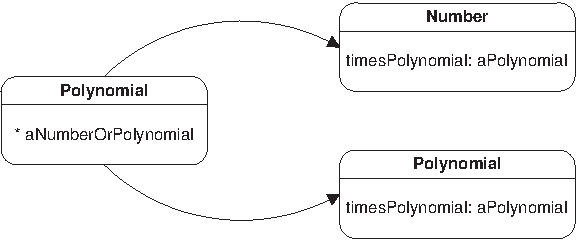
\includegraphics[width=8cm]{Figures/DoubleDispatching}
\caption{Triple dispatching}\label{fig:doubledispatch}
\end{figure}
It merely uses the fact that testing which class an object belongs
to is exactly what the virtual machine is doing when looking for
the code of the method corresponding to a message received by an
object. Thus, it is not necessary to repeat such test. Instead,
one delegates the execution of the method to the argument object.
as follows:
\begin{codeExample}
\begin{verbatim}

 * aNumberOrPolynomial
    ^ aNumberOrPolynomial timesPolynomial: self
\end{verbatim}
\end{codeExample}
In fact, the sending of the message {\tt timesPolynomial: self} to
the method's argument ensures that the types of both operands are
now completely known. One must now implement two versions of the
method {\tt timesPolynomial:}, one for instances of the class {\tt
DhbPolynomial} and one for the class {\tt Number}. Within both
versions of the method, the programmer can be sure that the type
of the argument is indeed an instance of class {\tt
DhbPolynomial}.

Figure \ref{fig:doubledispatch} shows this processus
schematically. Each box shows the class executing the method on
the top and the method with the type of the argument explicited at
the bottom. The arrows represent the sequence of execution.

One caveat with double dispatching is that the order of the
arguments is inverted. Thus, implementing double dispatching for
non commutative operators --- such as subtract, divide, or matrix
multiplication --- requires some thinking.

It is easy to understand that double dispatching is much faster
that testing the type of the argument. It only requires the
invocation of the operation message, whereas testing requires
evaluating the test itself plus a message invocation\footnote{{\tt
ifTrue:ifFalse:} {\it is} a message sent to the result of the
testing.}.

\section{Multiple dispatching}
\label{sec:multipledisp}The technique of double dispatching can be
extended to multiple levels. This is required when an operation is
implemented by a class having several subclasses, each subclasses
requiring a different behavior.

A good example of multiple dispatching is given by the addition
between matrices (\cf section \ref{sec:slinearalgebra}). The
product of two symmetric matrices is a symmetric matrix. In all
other cases, the result is a non-symmetric matrix.
\begin{figure}
\centering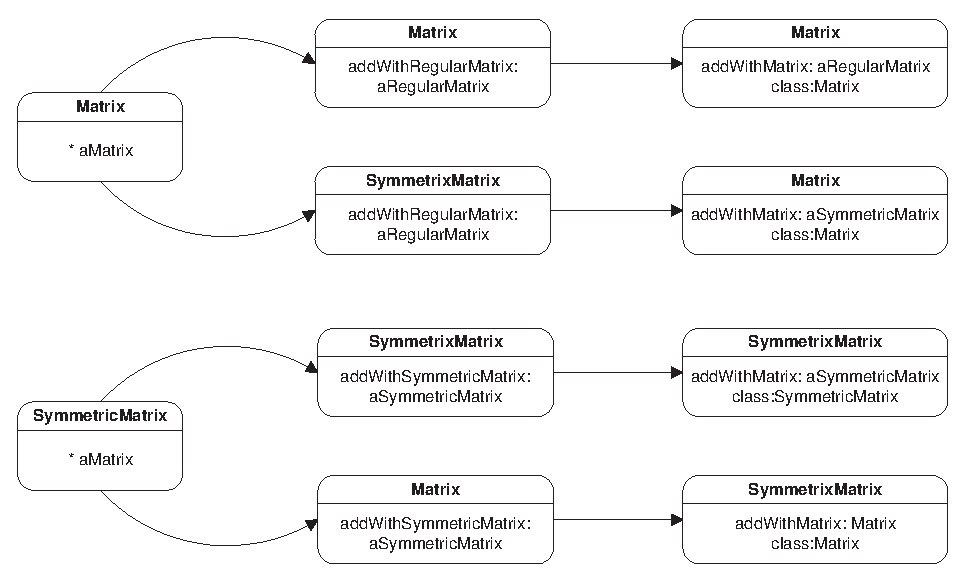
\includegraphics[width=8cm]{Figures/TripleDispatching}
\caption{Triple dispatching}\label{fig:tripledispatch}
\end{figure}
Thus, the addition operation is delegated a first time to the
proper subclass of the argument and a second time to the class of
the first operand. Here we have triple dispatching. This is shown
schematically in figure \ref{fig:tripledispatch}.

In the case of matrix multiplication, the situation is more
complex since the product is already being dispatched to
distinguish between three possible arguments. Here quadruple
dispatching is necessary.


\ifx\wholebook\relax\else\end{document}\fi
